% Created 2021-01-24 Sun 22:50
% Intended LaTeX compiler: pdflatex
\documentclass[11pt]{article}
\usepackage[utf8]{inputenc}
\usepackage[T1]{fontenc}
\usepackage{graphicx}
\usepackage{grffile}
\usepackage{longtable}
\usepackage{wrapfig}
\usepackage{rotating}
\usepackage[normalem]{ulem}
\usepackage{amsmath}
\usepackage{textcomp}
\usepackage{amssymb}
\usepackage{capt-of}
\usepackage{hyperref}
\usepackage{minted}
\hypersetup{colorlinks=true, linkcolor=black, filecolor=red, urlcolor=blue}
\usepackage[turkish]{babel}
\author{Eren Hatırnaz}
\date{14 Temmuz 2019}
\title{Yazılım Gündemi - 1\\\medskip
\large 8-14 Temmuz 2019}
\hypersetup{
 pdfauthor={Eren Hatırnaz},
 pdftitle={Yazılım Gündemi - 1},
 pdfkeywords={},
 pdfsubject={},
 pdfcreator={Emacs 27.1 (Org mode 9.3)},
 pdflang={Turkish}}
\begin{document}

\maketitle
\tableofcontents \clearpage\shorthandoff{=}

\begin{center}
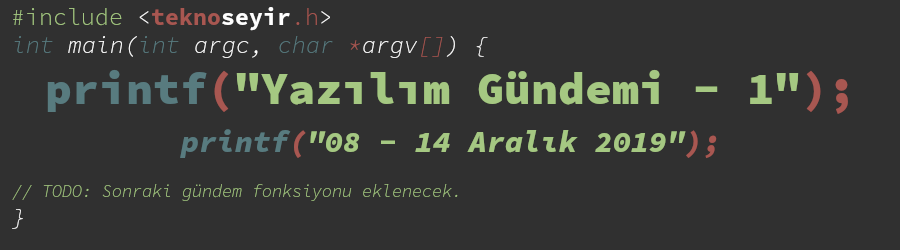
\includegraphics[width=.9\linewidth]{gorseller/yazilim-gundemi-banner.png}
\end{center}
\begin{center}
< Önceki Gündem | \textbf{8-14 Temmuz 2019} | \href{../02/yazilim-gundemi-02.pdf}{Sonraki Gündem >}

\href{https://teknoseyir.com/blog/yazilim-gundemi-1-08-14-temmuz-2019}{TeknoSeyir'de Oku}
\end{center}

Merhabalar,

TeknoSeyir'de en çok severek tükettiğim içerikler gündem değerlendirmeleri
(teknoloji, oyun ve bilim), özellikle de Haftalık Gündem Değerlendirmesi
videoları. Her ne kadar teknoloji ile ilgili haberleri değerlendiriyor olsalar
da, hitap ettikleri sadece yazılımcılar olmadığı için programlama ile ilgili
konulara fazla değinilmiyor. Ben de gün içerisinde sıkça HackerNews ve
Reddit'deki programlama kanallarını takip ettiğim için durdum ve dedim ki "e niye
ben yapmıyorum bu gündemi de, zaten bu tarz haberleri okumaya vakit ayırıyorum
hem kendim için bir arşiv olur hem de teknoseyir'deki yazılımcı arkadaşlara
faydalı olur" ve işte karşınızda bu haftanın yazılım gündemi.

Öncelikle şunu söylemeliyim ki: Bu gündem bütün bir haftada olan her şeyi kapsama
garantisi vermiyor. Karşıma çıkan haberlerden seçmeler yaparak, ilgilendiklerimi
yorumlayarak; pek bilgim olmadığı ya da değinilecek pek bir şeyinin olmadığı
konuları ise maddeler halinde yazarak yayınlayacağım bir seri olacak. Dolayısıyla
yazılımın her alanını, tüm konularını kapsamamı beklemeyin ama elimden geldiğince
çeşitli alanlardan maddeler toplamaya çalışacağım. Bir hevesle başlıyorum bakalım
umarım devam ettirebilirim.

Sizler de gündeme katkı sağlamak isterseniz yazılımın herhangi bir alanıyla
ilgili karşılaştığınız haberleri \#YazılımGündemineMalzeme etiketi ile
paylaşabilirsiniz. Etiketi takip edip oradan da haberleri eklemeye çalışacağım.

Silikon Vadisi sponsorluğunda hazırlanan Yazılım Gündemi başlıyor\ldots{}
\newpage
\section{\href{https://rubygems.org/gems/strong\_password/}{strong-password} isimli Ruby kütüphanesinin \href{https://withatwist.dev/strong-password-rubygem-hijacked.html}{arka kapı içerdiği ortaya çıktı}}
\label{sec:org10e59cb}
\begin{figure}[htbp]
\centering
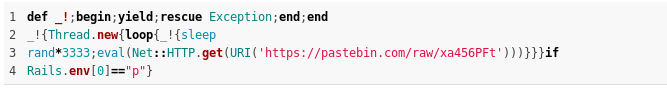
\includegraphics[width=.9\linewidth]{gorseller/strongpassword-ruby.png}
\caption{CVE Numarası: \href{https://nvd.nist.gov/vuln/detail/CVE-2019-13354}{CVE-2019-13354}}
\end{figure}

Tute Costa isimli kişi tarafından keşfedilen bu arka kapı sayesinde saldırgan
pastebin.com üzerinde tuttuğu bir kod parçasını çalıştırıyor ve sızdığı web
sitelerinin adreslerini öğrenmek için de özel bir alan adına GET isteği ile
birlikte sızılan web sitesinin URL adresini gönderiyor. Ruby ile yazılmış
popüler web framework sistemi olan Ruby on Rails'in de bir modülünde bu
kütüphanenin kullanılması güvenlik açığının boyutlarını büyük hale getiriyor.
Açığı bulan kişinin yaptığı araştırmaya göre, bu kütüphaneyi geliştiren kişinin
rubygems.org kullanıcı bilgileri çalınmış ve kütüphane saldırganın hesabına
geçmiş. Zaten bu nedenden dolayı github'daki sürümler ile rubygems.org'daki
sürümler uyuşmuyor. Bakıldığında github deposunda böyle bir kod bloğu
gözükmüyor ama rubygems.org'dan indirilen dosyalarda gözüküyor. Durumun farkına
varıldığında rubygems.org sitesi kütüphaneyi eski sahibine iade etti ve zararlı
kod parçaları kütüphaneden silindi. Açıktan etkilenmemek için yapmanız gereken
strong\_password kütüphanesini kullandığınız her projede 0.0.8 sürümüne
geçmeniz.

Kütüphanenin geliştiricisinin tahminine göre rubygems.org'daki kullanıcı
bilgilerinin çalınmasının nedeni başka birkaç sitede de kullandığı parola ile
aynı olması ve 2 adımlı doğrulamanın aktif olmaması -gerçi geliştirici bu
hesabı açtığında rubygems.org sitesi 2 adımlı doğrulama desteklemiyordu, o
konuda üzerine gitmek yanlış olur sanırım. Buradan çıkarılacak çok ders var.
Kullandığınız 3.parti kütüphanelere o kadar güvenmemek gerektiği, her yerde
aynı şifreyi kullanmamak ve adımlı doğrulamayı açmak gerektiği ilk aklıma
gelenler. Başka bir tartışma konusu da projelerimizin artık kocaman bir
"Bağımlılık Cehennemi"ne (Dependency Hell) dönüşmesi. En ufak ihtiyaçlar için
bile hemen 3.parti kütüphanelere, araçlara başvurmamız. Bunun başka bir
örneğini Azer Koçulu'nun \href{https://medium.com/eserozvataf/azer-ko\%25C3\%25A7ulu-kik-left-pad-ve-npm-ed7c3098ecfb}{leftpad olayında yaşamıştık} [konuyla ilgili kendisinin
de konuk olduğu \href{https://devpod.org/2016/03/28/036/}{bu podcast'i} mutlaka dinlemenizi tavsiye ederim]. Bakalım
geliştirici camiası olarak ne zaman dersimizi alacağız.

Trajikomik bir durum daha: Eğer Türkiye'deki sunucularda çalışan ve bu arka
kapının olduğu bir Ruby on Rails siteniz varsa, muhtemelen bu açıktan
etkilenmiyorsunuz çünkü pastebin.com sitesi ülkemizde 2012 yılından beri
yasaklı. Hükumetimiz sağ olsun web sitelerimizin güvenliğini de düşünüyor (!).
\section{Flutter 1.7 sürümü \href{https://medium.com/flutter/announcing-flutter-1-7-9cab4f34eacf}{duyuruldu}}
\label{sec:orgf650815}
\begin{itemize}
\item Yeni uygulamalar için \href{https://developer.android.com/jetpack/androidx}{AndroidX} desteği
\item OpenType zengin tipografi özellikleri
\item Oyun kontrolcüsü desteği
\item RangeSlider aracı
\item \href{https://developer.android.com/guide/app-bundle}{Android App Bundles}
\item Yeni örnekler ve dokumanlar
\item iOS üzerindeki yazı düzenleme özellikleri gelişti
\item 1250'nin üzerinde issue kapatıldı
\end{itemize}
\section{Go programlama dili topluluğu, \href{https://golang.org/}{dilin web sitesi}nden Google logosunu kaldırmayı \href{https://github.com/golang/go/issues/33021}{tartışıyor}}
\label{sec:org9c9bf56}
Daha doğrusu tartışamıyor desek yeridir. Çünkü Google çalışanları Github
üzerindeki tartışmayı \href{https://github.com/golang/go/issues/33021\#issuecomment-510981154}{yorum yapmaya kapattı} ve tartışmak isteyenleri mail
listesinden devam etmeye çağırdılar. Google çalışanının argümanı "biz bu
konuyu kendi içimizde konuştuk ve Go diline yatırım yapan, para harcayan ve
destekleyen bir şirket olduğumuz için logo'nun kalmasına karar verdik"
tarzında bir söylem oldu. Kaba tabirle "parasını verdik koyarız logo" demeye
getirseler de topluluğun argümanı şu şekilde oluyor: "Go dilini sadece Google
desteklemiyor, birçok destekleyen, yatırım yapan şirket var. O zaman onların
da logoları eklensin".

Üstelik bu, google ile go topluluğu arasındaki ilk tartışma da değil. Daha
önce de Google firmasının Go dili üzerindeki otoritesi \href{https://utcc.utoronto.ca/\~cks/space/blog/programming/GoIsGooglesLanguage}{şu yazı ile sorgulanmış}
ve ardından \href{https://news.ycombinator.com/item?id=19978200}{HackerNews} ve \href{https://www.reddit.com/r/programming/comments/brmxgf/go\_is\_googles\_language\_not\_the\_communitys/}{Reddit} gibi platformlarda tartışma devam etmişti. Bu
seferki tartışma da yine \href{https://www.reddit.com/r/programming/comments/ccidly/golang\_issue\_ticket\_remove\_the\_google\_logo/}{Reddit} gibi platformlarda devam ediyor.

Tekelleşen ve "Evil Corp" olma yolunda hızla ilerleyen Google önümüzdeki
zamanlarda daha çok tartışılmaya devam edecek gibi duruyor.
\section{TechEmpower, Web Frameworks Benchmarks \href{https://www.techempower.com/benchmarks/}{Round 18 yayınlandı}}
\label{sec:orga1a5c5c}
TechEmpower isimli firma belirli periyotlarda sürekli tekrarlanan, açık kaynak
olarak da \href{https://github.com/TechEmpower/FrameworkBenchmarks}{paylaşılan performans testleri} yapıyor. Toplamda 201 tane framework
sistemini test etmişler. Sonuçları biraz inceledim, açıkcası benim de ismini
hiç duymadığım onlarca framework var. İsmini bildiklerim az sayıda,
kullandıklarım ise bir elin parmaklarını geçmez o yüzden tabloyu pek
yorumlayamıyorum. Çoğu kategoride ilk sıralarda olanlardan hiç birini duymuş
ya da kullanmış değilim. Bunu sizin ilginize bırakıyorum.
\section{QuickJS JavaScript Motoru \href{https://bellard.org/quickjs/}{Yayınlandı}}
\label{sec:org9d81c22}
Fabrice Bellard isimli kişi tarafından yazılan bu JavaScript motoru küçük ve
gömülebilir (embeddable) olmasıyla öne çıkıyor. Ayrıca ECMAScript 2019
özelliklerinin tamamını destekliyor. Benim de ilgimi çekti ve indirip,
derleyip, denedim. 2-3 dakika sürdü derlenmesi. Daha sonra şöyle küçük bir
örnek yaptım. JavaScript'den çalıştırılabilir dosya elde etmek beni etkiledi
fakat tam olarak kullanım senaryosu nasıl olur bilemedim. \href{https://bellard.org/quickjs/quickjs.html}{Dokümantasyon}

\begin{figure}[htbp]
\centering
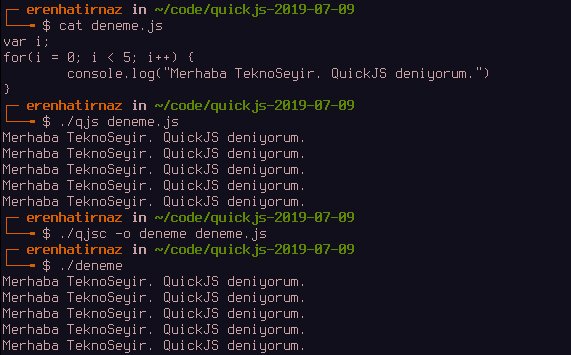
\includegraphics[width=.9\linewidth]{gorseller/quickjs-ts.png}
\caption{QuickJS Denemesi}
\end{figure}
\section{Uzak git deposu SourceHut, \href{https://drewdevault.com/2019/07/08/Announcing-annotations-for-sourcehut.html}{"Code Annotations" özelliğini duyurdu}}
\label{sec:orgbe14b61}
\begin{center}
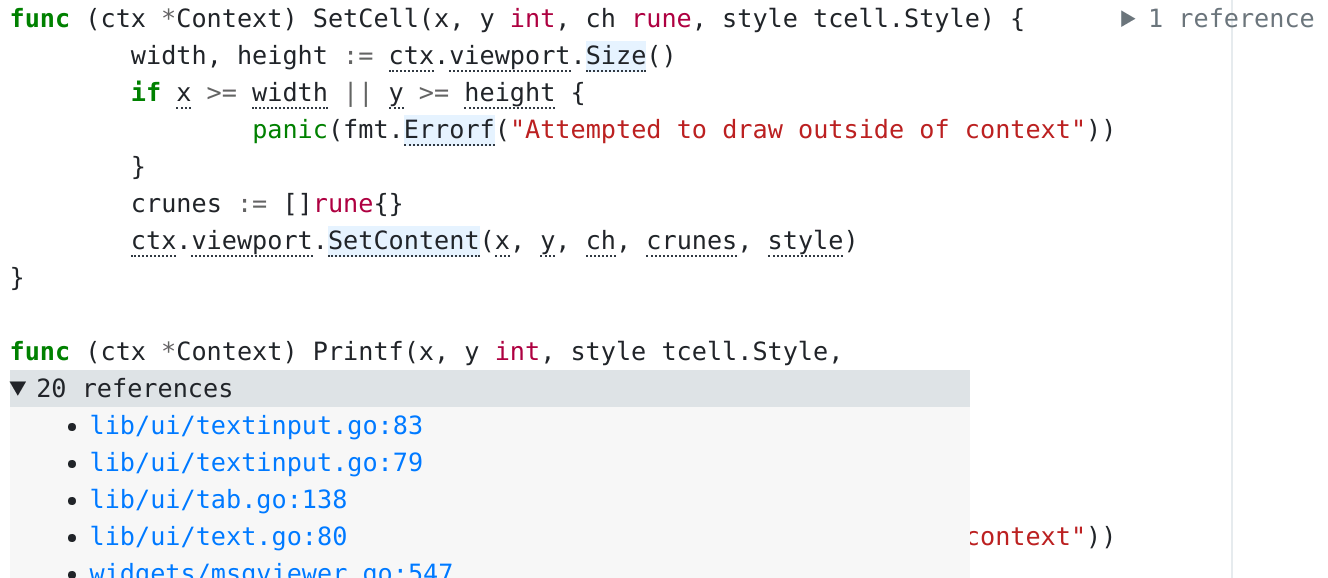
\includegraphics[height=4.5cm]{gorseller/sourcehut-ca.png}
\end{center}

SourceHut, \%100 açık kaynak uzak Git ve Mercurial deposu barındırma hizmeti
veren bir site. Aynı zamanda hata takip (issue tracker), e-posta listeleri ve
continuous integration sistemleri de mevcut.

Henüz sadece Go ve C dillerini (Python için de çalışıyormuş) destekleyen bu
özellik sayesinde bir fonksiyonun nerede tanımlandığını ya da tam tersi
fonksiyonun nerelerde kullanıldığını görebileceğiz. \href{https://git.sr.ht/\~mcf/cproc/tree/master/scan.c}{Örnek \{C\}}, \href{https://git.sr.ht/\~sircmpwn/aerc/tree/master/widgets/msgviewer.go}{Örnek \{Go\}},
\href{https://man.sr.ht/git.sr.ht/annotations.md}{Dokümantasyon}.

Geliştiricisi, "Favori programlama diliniz ile ilgili daha fazla şey öğrenmek
için güzel bir hafta sonu projesi olur" diyerek diğer diller için de
topluluktan destek beklediğini açıkladı.
\section{Diğer Haberler}
\label{sec:org83c959a}
\begin{itemize}
\item 2 Temmuz'da yaşanan Cloudflare sorununun \href{https://blog.cloudflare.com/details-of-the-cloudflare-outage-on-july-2-2019/}{detayları ortaya çıktı}.
\item Amazon, ekosistemine yeni bir hizmet ekliyor: \href{https://aws.amazon.com/tr/blogs/aws/amazon-eventbridge-event-driven-aws-integration-for-your-saas-applications/}{EventBridge}, \href{https://www.trek10.com/blog/amazon-eventbridge/}{Alternatif}.
\item Facebook, React Native uygulamaları için özel olarak optimize edilmiş Hermes
isimli JavaScript motorunu \href{https://hermesengine.dev/}{açık kaynak hale getirdi}, \href{https://github.com/facebook/hermes}{GitHub deposu},
\href{https://facebook.github.io/react-native/docs/hermes/}{Dokümantasyon}.
\item Uber, H3 isimli mekansal (geospatial) indeksleme sistemini \href{https://eng.uber.com/visualizing-city-cores-with-h3/}{açık kaynak hale
getirdi}, \href{https://github.com/uber/h3}{GitHub deposu}.
\item Firefox 68 sürümünde, mikrofon ve kamera erişimi isteyen siteler için \href{https://blog.mozilla.org/webrtc/camera-microphone-require-https-in-firefox-68/}{https
olma zorunluluğu geldi}.
\item Microsoft, Quantum Development Kit'i (QTK) \href{https://cloudblogs.microsoft.com/quantum/2019/07/11/microsoft-quantum-oss-available-github/}{açık kaynak hale getirdi},
\href{https://docs.microsoft.com/tr-tr/quantum/install-guide}{Dokümantasyon}.
\item Kendi başına uçabilen drone'lar için açık kaynak platform: \href{https://www.gaas.dev/}{GAAS}, \href{https://github.com/generalized-intelligence/GAAS}{GitHub
Deposu}.
\item Slack alternatifi Mattermost, 50 milyon dolarlık \href{https://venturebeat.com/2019/06/19/mattermost-raises-50-million-to-advance-its-open-source-slack-alternative/}{yatırım aldı}.
\item Tip-korumalı yeni bir programlama dili: \href{https://github.com/mirth-lang/mirth}{mirth}.
\item Tarayıcı tabanlı .NET uygulamaları için yeni bir web framework duyuruldu:
\href{https://www.youtube.com/watch?v=uW-Kk7Qpv5U}{Blazor}.
\item Google Tablolar'ı veritabanı olarak kullanmaya olanak sağlayan açık kaynaklı
bir hizmet çıktı: \href{https://steinhq.com/}{Stein}, \href{https://github.com/SteinHQ}{GitHub sayfası}.
\item Elements isimli C++ GUI kütüphanesi \href{https://www.cycfi.com/2019/07/photon-micro-gui/}{açık kaynak olarak yayınlandı}, \href{https://github.com/cycfi/elements}{GitHub
Deposu}.
\item RestQL V3 sürümü \href{https://www.infoq.com/news/2019/07/restql-v3-released/}{yayınlandı}.
\item ReactPHP ilk stabil sürümü 1.0.0'ı \href{https://github.com/reactphp/react/releases/tag/v1.0.0}{çıkardı}.
\item FreshIDE 2.7.0 sürümü \href{https://fresh.flatassembler.net/index.cgi?page=content/2\_download.txt}{çıktı}.
\item GammaRay 2.11.0 sürümü \href{https://www.kdab.com/gammaray-2-11-0-release/}{çıktı}.
\item OpenAPI Generator 4.0.3 sürümü \href{https://github.com/OpenAPITools/openapi-generator/releases/tag/v4.0.3}{çıktı}.
\item KDE Frameworks 5.60.0 sürümü \href{https://kde.org/announcements/kde-frameworks-5.60.0.php}{çıktı}.
\end{itemize}
\section{Lisans}
\label{sec:org74b7bd4}
\begin{center}
\begin{center}

\includegraphics[height=1.5cm]{../../../img/CC_BY-NC-SA_4.0.png}
\end{center}

\href{yazilim-gundemi-01.pdf}{Yazılım Gündemi - 1} yazısı \href{https://erenhatirnaz.github.io}{Eren Hatırnaz} tarafından \href{http://creativecommons.org/licenses/by-nc-sa/4.0/}{Creative Commons
Atıf-GayriTicari-AynıLisanslaPaylaş 4.0 Uluslararası Lisansı} (CC BY-NC-SA 4.0)
ile lisanslanmıştır.
\end{center}
\end{document}
